% compile: $ pdflatex group.tex

% TODO:
%
% SOME MARGIN FIGURES ARE DROPPING OFF THE PAGE
% JUST A WEE SUGGESTION THAT THIS SHOULD BE FIXED
% BEFORE WE SUBMIT

\documentclass[a4paper, notoc]{tufte-handout}

\title{Human Computer Interaction\\ Coursework 2 Report}

\author{Group 35}

%\date{1st January 1970} % without \date command, current date is supplied

%\geometry{showframe} % display margins for debugging page layout
\usepackage[utf8]{inputenc}
\usepackage{appendix}
\usepackage{graphicx} % allow embedded images
\setkeys{Gin}{width=\linewidth,totalheight=\textheight,keepaspectratio}
\graphicspath{{graphics/}} % set of paths to search for images
\usepackage{amsmath}  % extended mathematics
\usepackage{booktabs} % book-quality tables
\usepackage{units}    % non-stacked fractions and better unit spacing
\usepackage{multicol} % multiple column layout facilities
\usepackage{lipsum}   % filler text
\usepackage{fancyvrb} % extended verbatim environments\
\fvset{fontsize=\normalsize}% default font size for fancy-verbatim environments

\let\origdescription\description
\renewenvironment{description}{
  \setlength{\leftmargini}{1.5em}
  \origdescription
  \setlength{\itemindent}{-1.5em}
  \setlength{\labelsep}{\textwidth}
}
{\endlist}


\begin{document}
\maketitle % this prints the handout title, author, and date
\vspace{1em}
\noindent
\begin{tabular}{l r}
  Chris Campbell & s1334028\\
  Karel Kuzmiak  & s1334628\\
  Angus Pearson  & s1311631\\
  Ben Shaw       & s1338564\\
\end{tabular}

%\tableofcontents
%\newpage

\section{Concept}\label{sec:concept}

\begin{marginfigure}
  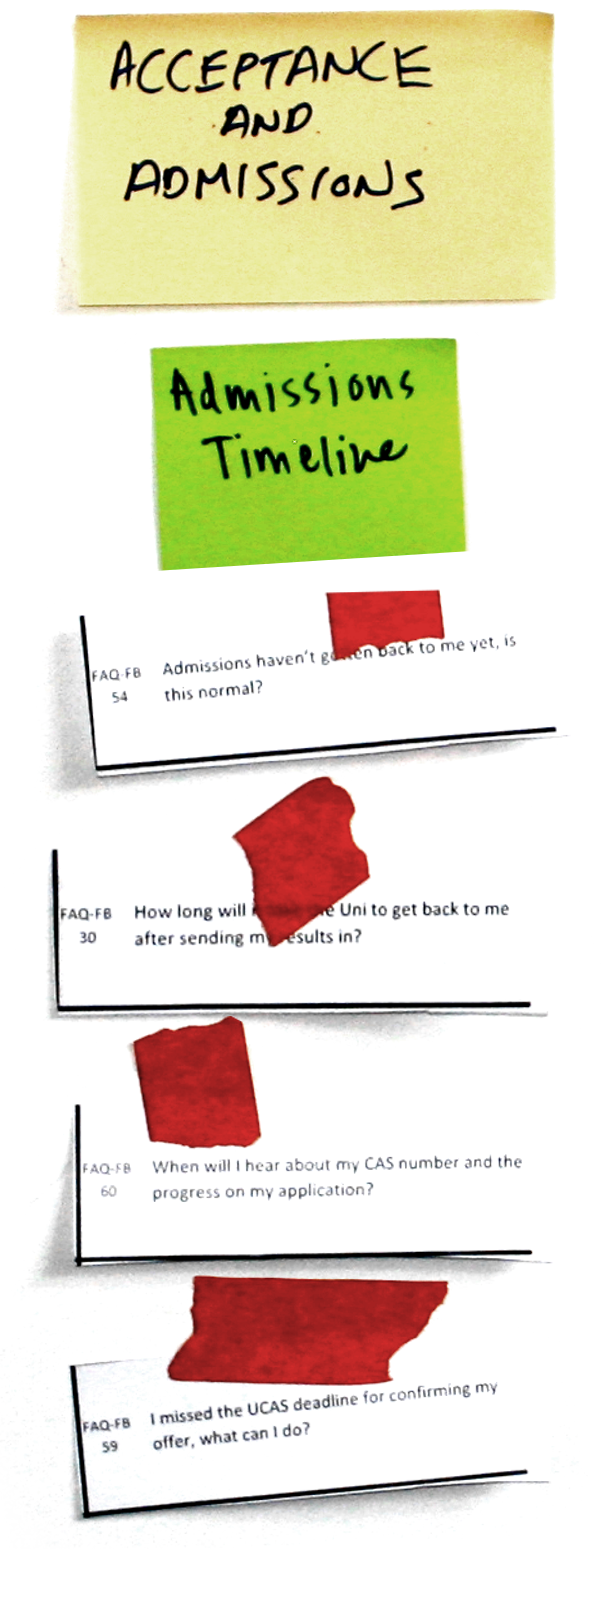
\includegraphics{acceptance_admissions_affinity.png}
  \caption{
    \label{fig:accept-admit-affinity}
    A section of an Affinity Diagram, where all the questions about admissions relate to the timing of admissions. Other qustions in the `Acceptance and Admissions' group pertained to meeting conditions and the post-decision process.}
\vspace{1em}
\end{marginfigure}

The affinity diagrams produced by the tutorial groups suggest that the questions asked could easily be mapped chronologically in the lead up to, and immediately after, starting at the University of Edinburgh. Following from that, we propose an interface centred on a timeline, with information arranged in cards sequentially placed along a vertically descending line. Iconography down the timeline allows quick scanning and recognition, with the icon roundel being clickable, to mark the accompanying content card as \textit{done}
\footnote{In this case \textit{done}, is rather abstract; meaning completed or no longer requiring the user's attention}


\section{Design Justification}\label{sec:design-justification}

Our colour scheme consists of three primary colours: pink, consistent with the University's branding for Fresher's week; blue, a colour used heavily by the University's welcome literature; and green, which is a commonly used colour indicative of positive progress or success.

Continuing to adhere to the University's design guidelines, our design makes use of the \textit{Crimson Text} and \textit{Source Sans Pro} fonts.

Upon loading the page, users are greeted by an illustrated \textit{hero image} of the University's Old College. The hero serves as a clear call to action above the fold, and grounds content below -- stating what the page it is, who it is for and what it contains. Beneath the fold begins the timeline that has \textit{cards}\footnote{Inspired by the \textit{Material Design} paradigm, a drop shadow drawn from below the card mimics that of physical paper's interaction with light.} spread out in a \textit{zigzag} fashion, centring the user's focus on one item at a time whilst creating a vertical progression that logically follows from the content's temporal nature. Each card is signposted by an \textit{icon} which alludes to it's content and topic. \textit{Buttons} were opted for over plain hyperlinks, following the belief that buttons afford clickability more than a traditional blue hyperlink. Further to this buttons hold more visual weight and from a usability perspective present a larger touch target on smaller, touchscreen devices.


% Users aren't affraid to scroll --> Justifies super long single page
% https://www.clicktale.com/academy/blog/unfolding-the-fold-insights-into-webpage-scroll/
%
% 91% of the page-views had a scroll-bar.
% 76% of the page-views with a scroll-bar, were scrolled to some extent.
% 22% of the page-views with a scroll-bar, were scrolled all the way to the bottom.

\section{Interaction Design}\label{label:interaction-design}

Our team chose to implement the \textit{instructing and manipulating} interactions on our webpage. TODO: GIVE EXAMPLE OF WHERE IN DESIGN Early versions of the webpage held an attempt at conversing with the user by prompting them on arrival with an \textit{instant messaging} conversational form, with the hope of gauging what type of student they are. It had been hoped that this would allow for the page to be tailored in accordance with that particular student's needs. For example, hiding information regarding visas to students who already reside in the UK or Éire, yet displaying it those who live elsewhere. This feature was ultimately scrapped as it proved to be complex to implement within our given time frame, and given it's dependance on persistent state, out of scope.

TODO: Tour justification, reasoning and explain

\section{Usability Testing}\label{sec:usability-testing}

\subsection{A/B Testing}\label{subsec:a-b-testing}

To conduct an \textit{A/B} test, two different versions of the webpage were created -- \textit{A}'s design utilised the aforementioned timeline format; the \textit{challenger} \textit{B} design instead presented a more conventional tiled card formation. These variants are shown in Figures \ref{fig:avariant} and \ref{fig:bvariant}.

Analysis of the test was carried out with \textit{Google Analytics' A/B Testing facility}. Respondents were randomly served with either the \textit{A} or \textit{B} variant; subsequently their time spent on the page was recorded and a link to an optional survey produced at the bottom of page.

The results from the survey, consisting of the more than \emph{60} responses received, showed a strong preference towards the \textit{A} version of the website. Specifically, respondents generally found that the linear chronological form was easier to navigate and proved to be more effective at clearly displaying the information.

\begin{marginfigure}
  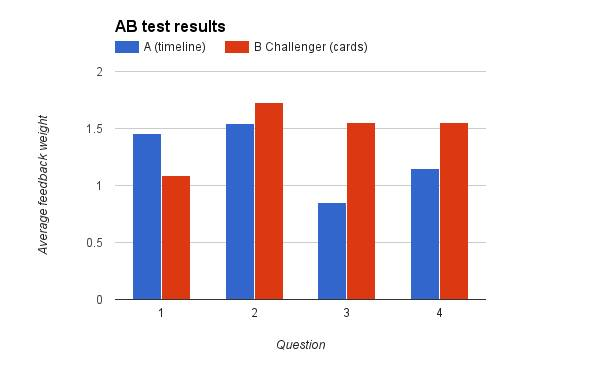
\includegraphics[width=\linewidth]{abresults.png}
  \caption{
    \label{fig:abresults}
    Results of the \textit{A/B Testing} showed that while both variants were easy to navigate, respondents thought of the \textit{A Variant} as being more efficient with its usage of space and more aesthetically pleasing.
  }
\end{marginfigure}

TODO: Substantiate claims

TODO: Quotes

TODO: Survey Figure

\begin{marginfigure}
  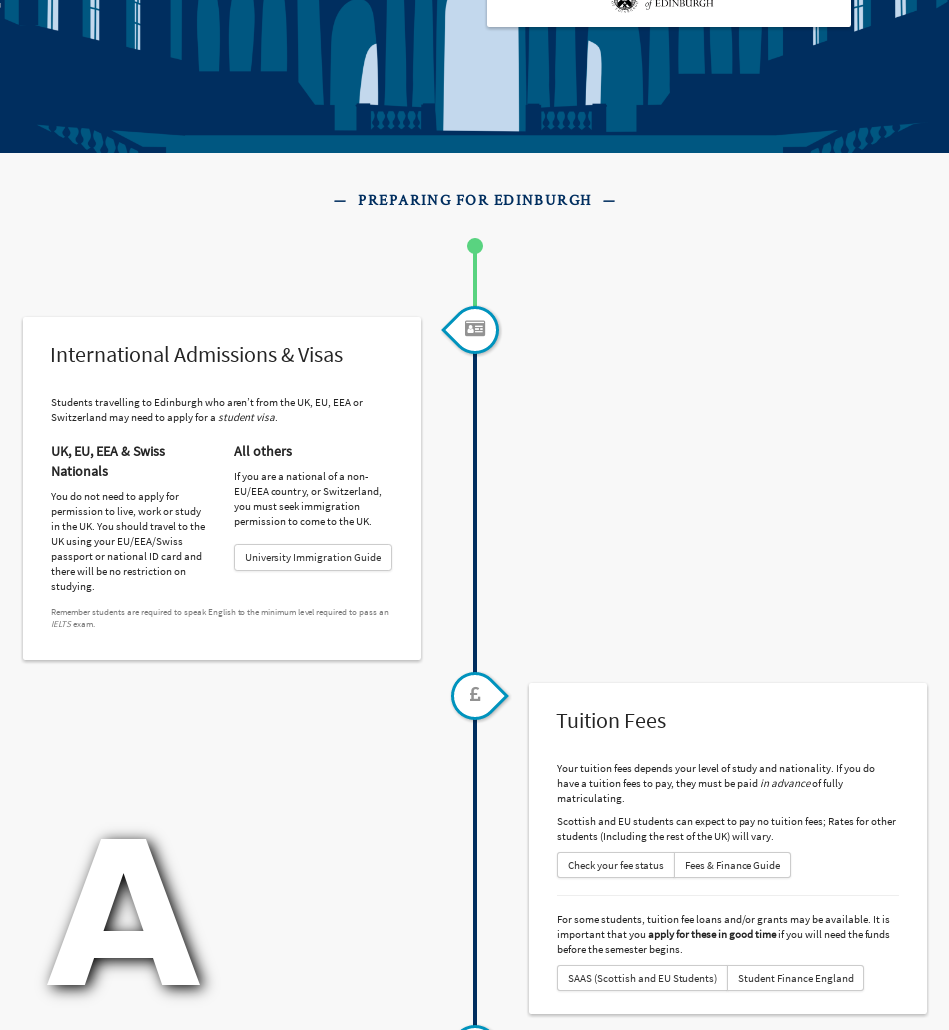
\includegraphics[width=\linewidth]{avariant.png}
  \caption{
    \label{fig:avariant}
    Screencapture showing \textit{A Variant} from \textit{A/B Testing}.
  }

\end{marginfigure}

\begin{marginfigure}
  
\includegraphics[width=\linewidth]{bvariant.png}
  \caption{
    \label{fig:bvariant}
    Screencapture showing \textit{B Variant} from \textit{A/B Testing}.
  }

\end{marginfigure}

\subsection{Informal Interview}\label{subsec:interview}

% Reasoning behind why the website is usable. This section will likely include 
% the outcome of any evaluations you conducted. Unlike the last coursework I do 
% not expect you to do a full formal analysis and description. A few sentences 
% on the method you used is fine. The key is providing reasoning on either why 
% the site is usable, or what you changed to make it so.

Tutorials to informally interview tutors to get feedback on the interface and concept throughout different stages of development. Broad questions were prepared before the evaluations and hand written notes were taken of the feedback given back. Several design changes were made following the feedback which helped lead to an improved product.

\section{Reflection}

% Reflection paragraph: what you have learned from completing this coursework. 
% What worked, what didn't, and if you could go back and do this coursework 
% again what might you do differently the next time.

Upon completion the of web implementation we realised that a huge aid to us as a group had been the robustness and relatively small learning curve of \textit{Bootstrap}. \textit{Bootstrap} allowed for us to refine and expand upon previously existing templates, producing a webpage boasting a responsive design. Undertaking the implementation phase in this manner allowed for the team to spend more time developing our test phase and the subsequent write up. Mostly as a result of time-constraints and the nature of the task the interaction design \& UI lack polish, with some interactions (most notably the Next \& Previous buttons) behaving in a simpler or less intuitave way than hoped. Yet, in the face of the already positive feedback it was decided to develop the webpage no further.

One request raised within feedback was for the webpage to remember stateful information. Our team had hoped to implement this, as it would have been exceedingly beneficial to new students looking to continuously monitor their progress before and immediately after starting University, however we deem developing a backend out of scope. If this were to be developed, it would tie in to the core element that is the timeline and embolden the page's theme of chronological progression.


\section{Tools and Templates}

%% REQUIREMENTS %%
% A list of any tools or templates you used to construct the website.

\begin{description}

\item[Jekyll]
Static site generator written in Ruby. Supports Markdown for 
content markup and the \textit{SASS} CSS pre-processor.
Hosting provided by GitHub pages.
\\
\href{http://jekyllrb.com/}{http://jekyllrb.com/}

\item[BootStrap]
Web UI framework (CSS, JavaScript) freely available, created by Twitter.
\\
\href{http://getbootstrap.com/}{http://getbootstrap.com/}

\item[FontAwesome]
Web Icon set, freely available.
\\
\href{http://fontawesome.io/}{http://fontawesome.io/}


\item[JQuery]
JavaScript frontend library
\\
\href{https://jquery.com/}{https://jquery.com/}

\item[University of Edinburgh Style Guide]
Fonts -- Serif:- \textit{Crimson Text}, Sans-Serif: \textit{Source Sans Pro} both 
available as \href{https://fonts.google.com/}{Google Web Fonts}.
\\
Colours are taken from 
\href{http://www.ed.ac.uk/communications-marketing/resources}{\textit{Brand Guidelines}} 
and associated pages.
\\



\end{description}




\section*{Group Mark Allocation}\label{group-mark-allocation}
%% REQUIREMENTS %%

% How the group would like me to allocate marks. Two options: 1) everybody gets 
% the same mark, 2) a clear list of who is responsible for which part of the 
% website or evaluation. In the case of #2 10 points will be marked group wide 
% for the general design of the website and the remaining 40 points will be marked 
% based on the individual portion of the work.

We wish for allocated marks to be identical for each member of our team.

\end{document}

